%!TEX TS-program = xelatex
%!TEX encoding = UTF-8 Unicode
% Awesome CV LaTeX Template for CV/Resume
%
% This template has been downloaded from:
% https://github.com/posquit0/Awesome-CV
%
% Author:
% Claud D. Park <posquit0.bj@gmail.com>
% http://www.posquit0.com
%
% Template license:
% CC BY-SA 4.0 (https://creativecommons.org/licenses/by-sa/4.0/)
%


%-------------------------------------------------------------------------------
% CONFIGURATIONS
%-------------------------------------------------------------------------------
% A4 paper size by default, use 'letterpaper' for US letter
\documentclass[11pt, a4paper]{awesome-cv}

% Configure page margins with geometry
\geometry{left=1.4cm, top=.8cm, right=1.4cm, bottom=1.8cm, footskip=.5cm}

% Specify the location of the included fonts
\fontdir[fonts/]

% Color for highlights
% Awesome Colors: awesome-emerald, awesome-skyblue, awesome-red, awesome-pink, awesome-orange
%                 awesome-nephritis, awesome-concrete, awesome-darknight
\colorlet{awesome}{awesome-red}
% Uncomment if you would like to specify your own color
% \definecolor{awesome}{HTML}{CA63A8}

% Colors for text
% Uncomment if you would like to specify your own color
% \definecolor{darktext}{HTML}{414141}
% \definecolor{text}{HTML}{333333}
% \definecolor{graytext}{HTML}{5D5D5D}
% \definecolor{lighttext}{HTML}{999999}

% Set false if you don't want to highlight section with awesome color
\setbool{acvSectionColorHighlight}{true}

% If you would like to change the social information separator from a pipe (|) to something else
\renewcommand{\acvHeaderSocialSep}{\quad\textbar\quad}


% -------------------------------------------------------------------------------
%       PERSONAL INFORMATION
%       Comment any of the lines below if they are not required
% -------------------------------------------------------------------------------
% Available options: circle|rectangle,edge/noedge,left/right
% \photo[rectangle,edge,right]{./examples/profile}
\name{Samuel T.}{Jahnke}
% \position{Software Architect{\enskip\cdotp\enskip}Security Expert}
% \address{42-8, Bangbae-ro 15-gil, Seocho-gu, Seoul, 00681, Rep. of KOREA}

\mobile{(+507)399-6195}
\email{samueljahnke6@gmail.com}
%% \homepage{www.castles.life}
\github{asamwow@github.com}
% \linkedin{posquit0}
% \gitlab{gitlab-id}
% \stackoverflow{SO-id}{SO-name}
% \twitter{@twit}
% \skype{skype-id}
% \reddit{reddit-id}
% \medium{madium-id}
% \googlescholar{googlescholar-id}{name-to-display}
%% \firstname and \lastname will be used
% \googlescholar{googlescholar-id}{}
% \extrainfo{extra informations}

\quote{Show me your moves  -- Captain Falcon}

\begin{picture}(50,50)
\put(420,-110){\hbox{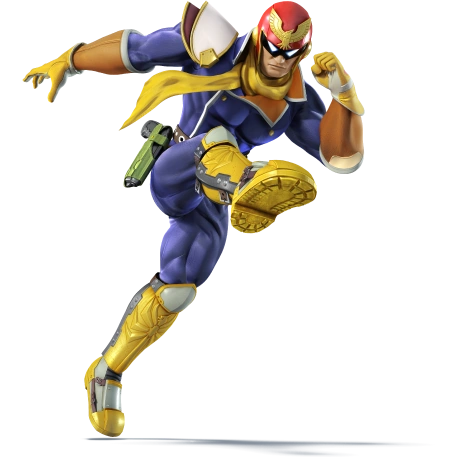
\includegraphics[scale=0.2]{./examples/falcon.png}}}
\end{picture}

%-------------------------------------------------------------------------------
\begin{document}

% Print the header with above personal informations
% Give optional argument to change alignment(C: center, L: left, R: right)
\makecvheader

% Print the footer with 3 arguments(<left>, <center>, <right>)
% Leave any of these blank if they are not needed
%% \makecvfooter
%%   {\today}
%%   {View this LaTeX document at github.com/asamwow/Awesome-CV}
%%   {}

%-------------------------------------------------------------------------------
%       CV/RESUME CONTENT
%       Each section is imported separately, open each file in turn to modify content
%-------------------------------------------------------------------------------
%-------------------------------------------------------------------------------
%       SECTION TITLE
%-------------------------------------------------------------------------------
\cvsection{Experience}


%-------------------------------------------------------------------------------
%       CONTENT
%-------------------------------------------------------------------------------
\begin{cventries}

%---------------------------------------------------------
  \cventry
    {Castles} % Organization
    {Game Developer} % Job title
    {Albert Lea, Minnesota} % Location
    {September 2022 - Present} % Date(s)
    {
      \begin{cvitems} % Description(s) of tasks/responsibilities
        \item {Sole developer of \url{http://castles.life}.}
        \item {Graphics, multiplayer, hosting, identity system, map editor, animations, models, mod support.}
      \end{cvitems}
    }

%---------------------------------------------------------


%---------------------------------------------------------
  \cventry
    {Public and Private} % Organization
    {Substitute Teacher} % Job title
    {Various Locations} % Location
    {Aug 2022 - May 2023} % Date(s)
    {
      \begin{cvitems} % Description(s) of tasks/responsibilities
        \item {Introduced text based programming to middle school students.}
        \item {Used patience and empathy to support children with ASD.}
      \end{cvitems}
    }

%---------------------------------------------------------
  \cventry
    {Stratagem Group} % Organization
    {Software Developer} % Job title
    {King of Prussia, Pennsylvania} % Location
    {Jan 2022 - Apr 2022} % Date(s)
    {
      \begin{cvitems} % Description(s) of tasks/responsibilities
        \item {Automated development pipeline with makefiles, systemd unit files, lisp, and literate org-mode markdown documentation.}
      \end{cvitems}
    }

%---------------------------------------------------------
  %% \cventry
  %%   {Mathnasium} % Organization
  %%   {Math Tutor} % Job title
  %%   {Rosemont/Blue Bell, Pennsylvania} % Location
  %%   {Dec. 2021 - Apr 2022} % Date(s)
  %%   {
  %%     \begin{cvitems} % Description(s) of tasks/responsibilities
  %%       \item {Understand students perspective by being a patient listener to understand how to help them best.}
  %%       \item {Encourage general understanding of concepts by asking many questions and creating unique problems or diagrams.}
  %%     \end{cvitems}
  %%   }

  \cventry
    {Lockheed Martin - Space} % Organization
    {Software Engineer Asc.} % Job title
    {King of Prussia, Pennsylvania} % Location
    {Sept. 2020 - Dec. 2021} % Date(s)
    {
      \begin{cvitems} % Description(s) of tasks/responsibilities
        \item {Automated development procedures such as kubernetes and gitlab pipelines with makefiles, bash, and python scripts.}
        \item {Worked with my team to accomplish various features within time limitations.}
      \end{cvitems}
    }

%---------------------------------------------------------
  \cventry
    {HVH Precision Analytics} % Organization
    {Web Developer} % Job title
    {Wayne, Pennsylvania} % Location
    {Nov. 2019 - Apr. 2020} % Date(s)
    {
      \begin{cvitems} % Description(s) of tasks/responsibilities
        \item {Worked with Amazon AWS resources to query medical patient data and run analytics.}
        \item {Helped develop localized testing environment with mimicked network connections and user inputs.}
      \end{cvitems}
    }

%% %---------------------------------------------------------
%%   \cventry
%%     {Mathnasium/Private Lessons} % Organization
%%     {Math Tutor} % Job title
%%     {Menomonie, Wisconsin} % Location
%%     {Mar. 2016 - Present} % Date(s)
%%     {
%%       \begin{cvitems} % Description(s) of tasks/responsibilities
%%         \item {Understand students perspective by being a patient listener to understand how to help them best.}
%%         \item {Encourage general understanding of concepts by asking many questions and creating unique problems or diagrams.}
%%         \item {Displayed skills in calculus and linear algebra by breaking down advanced mathematical concepts to a less technical audience.}
%%       \end{cvitems}
%%     }

%% %---------------------------------------------------------
  \cventry
    {Shotgun Express, Inc}
    {Web Developer}
    {Twin Cities, Minnesota} % Location
    {Fall 2018} % Date(s)
    {
      \begin{cvitems} % Description(s) of tasks/responsibilities
        \item {Created delivery price calculator in javascript.}
      \end{cvitems}
    }

%---------------------------------------------------------

\end{cventries}

%-------------------------------------------------------------------------------
%	SECTION TITLE
%-------------------------------------------------------------------------------
\cvsection{Skills}


%-------------------------------------------------------------------------------
%	CONTENT
%-------------------------------------------------------------------------------
\begin{cvskills}

%---------------------------------------------------------
  \cvskill
    {Programming} % Category
    {C/C++, C\#, Java, Python, HTML, Javascript, Bash, LaTeX}

%---------------------------------------------------------
  \cvskill
    {Software} % Category
    {Linux, Git, Emacs, Unity 3D} % Skills

%---------------------------------------------------------
  \cvskill
    {Projects} % Category
    {OpenGL, Databases, AI, Inverse Kinematics} % Skills

%---------------------------------------------------------

\end{cvskills}

%-------------------------------------------------------------------------------
%	SECTION TITLE
%-------------------------------------------------------------------------------
\cvsection{Education}


%-------------------------------------------------------------------------------
%	CONTENT
%-------------------------------------------------------------------------------
\begin{cventries}

%---------------------------------------------------------
  \cventry
  {B.S. in Applied Math and Computer Science} % Degree
  {California Polytechnic State University} % Institution
  {San Luis Obispo, California} % Location
  {Expected Summer 2019} % Date(s)
  {
    \begin{cvitems} % Description(s) bullet points
      \item {3.86 GPA}
    \end{cvitems}
  }

%---------------------------------------------------------
\end{cventries}

%-------------------------------------------------------------------------------
\end{document}
